\begin{figure}
    \begin{center}
    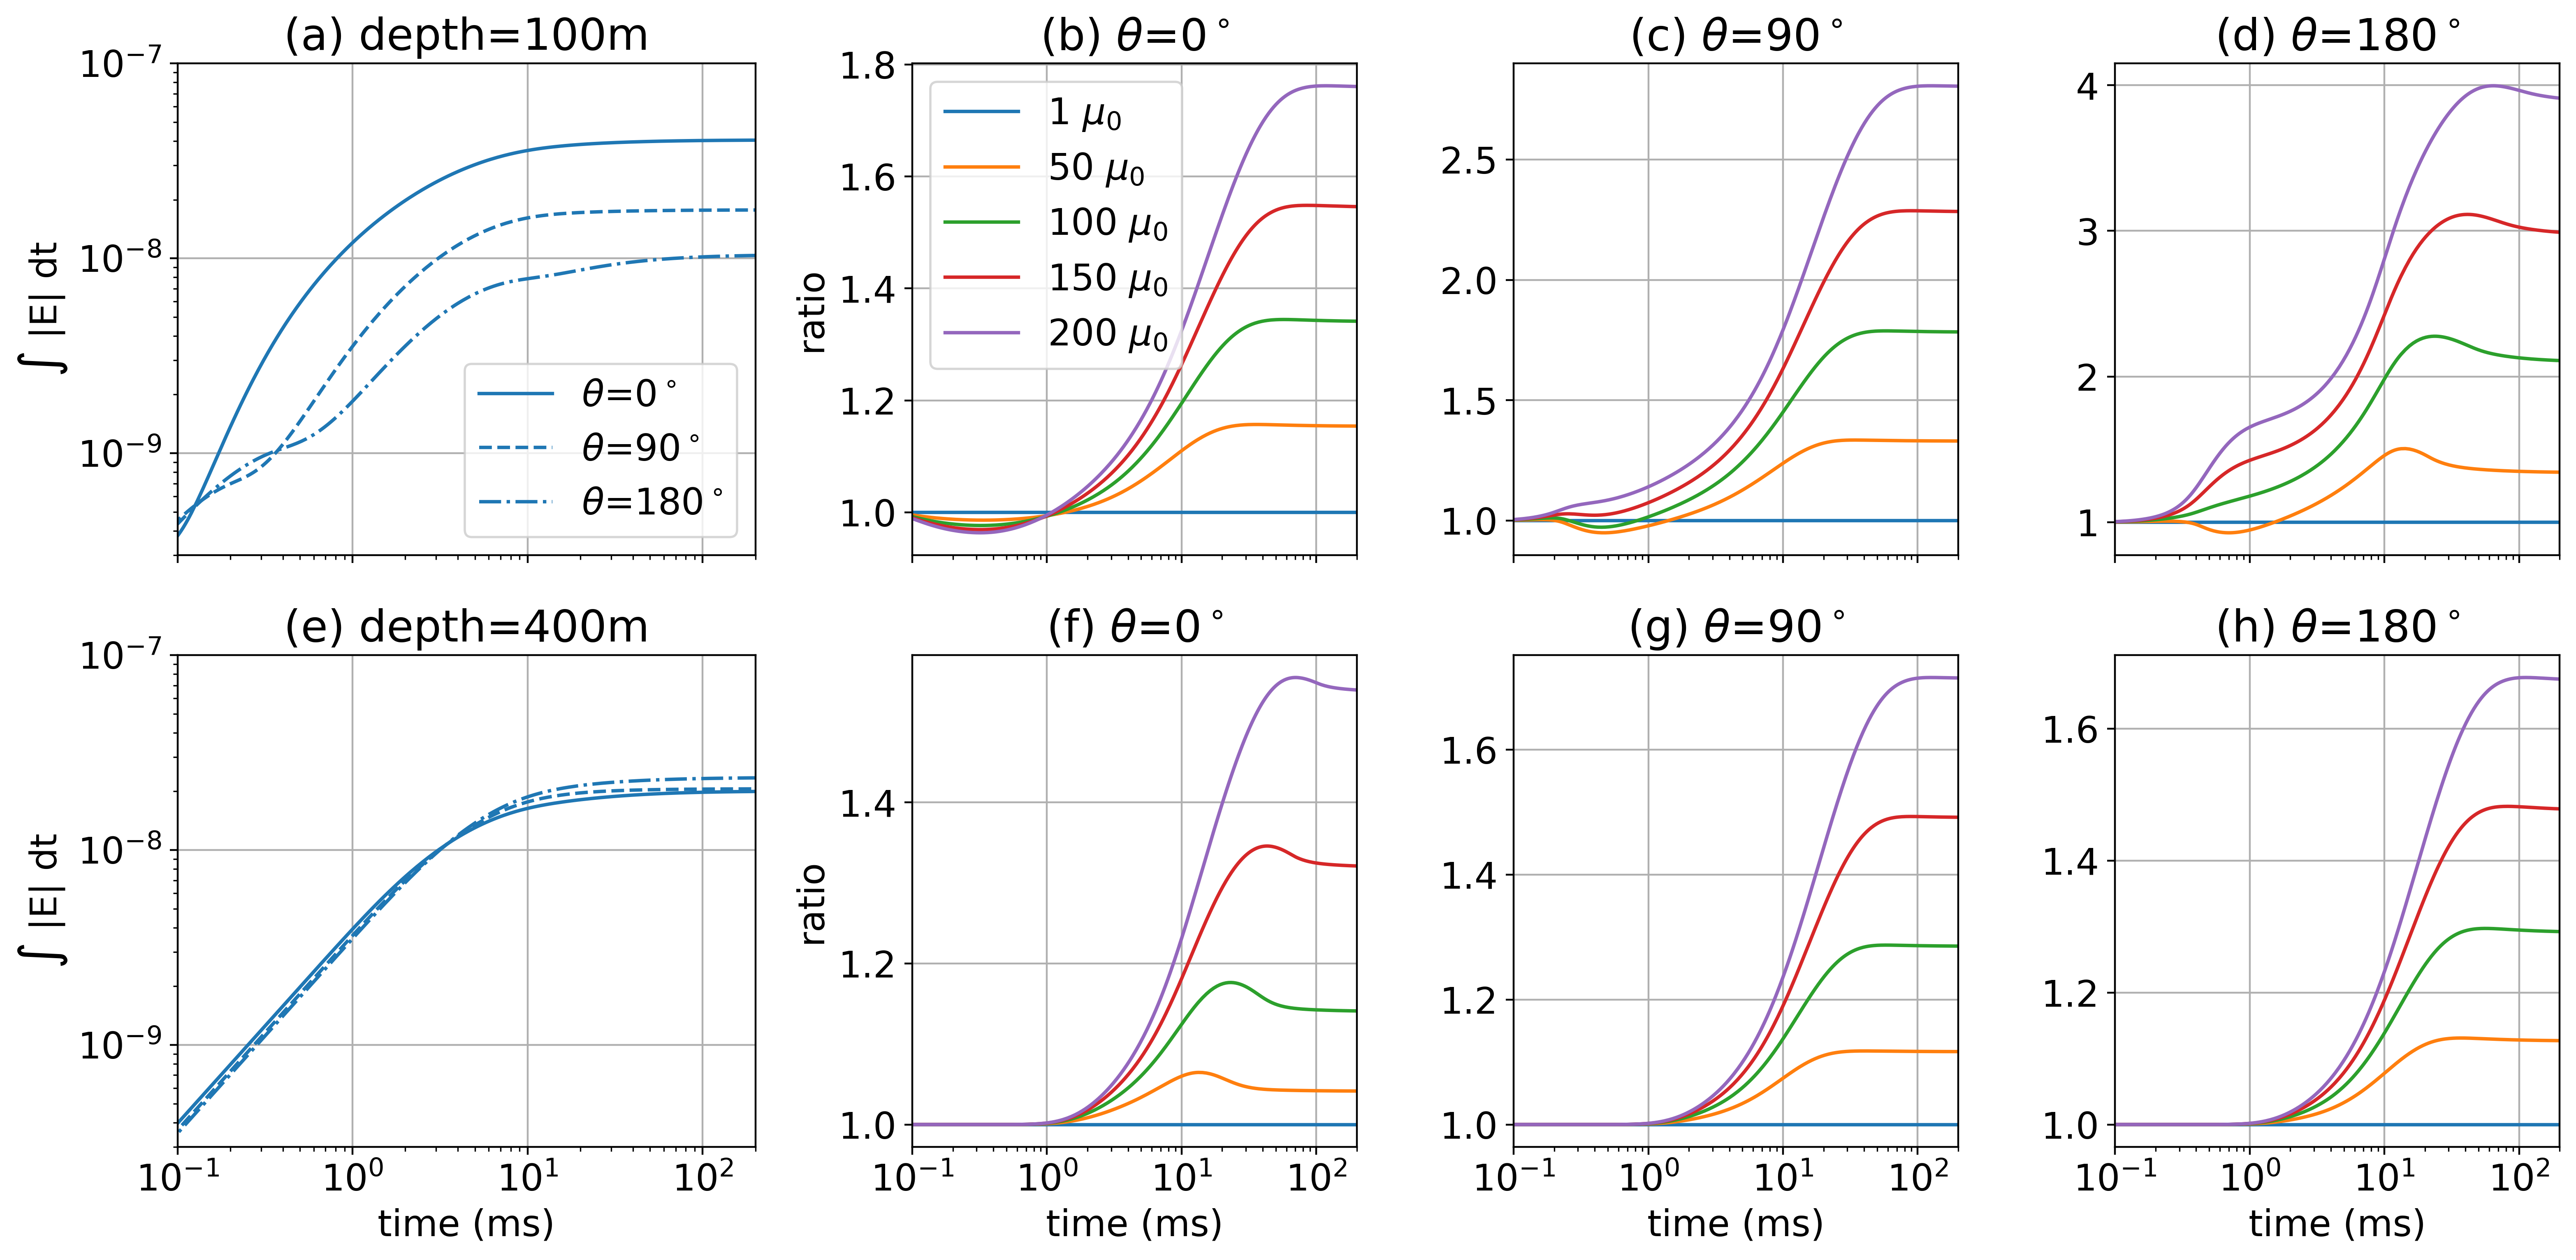
\includegraphics[width=\textwidth]{figures/excitation-time-integrated.png}
    \end{center}
\caption{
    Integral of the average electric field in a test volume through time, which we use as a proxy for excitation. The test volume extends from 50m - 100m radially and 50m vertically centered about depths of (a) 100m and (e) 400m. The different line-styles in (a) and (e) indicate different azimuths ($0^\circ$ is under the transmitter wire, $90^\circ$ is orthogonal to it, and $180^\circ$ is opposite to it) for the non-permeable well ($\mu=\mu_0$). Panels (b), (c), and (d) show the ratio of the excitation with respect to the non-permeable well ($\mu=\mu_0$) for the test volume centered at 100m depth. Panels (f), (g) and (h) show the ratios of the excitation for the test volume centered at 400m depth.
}
\label{fig:excitation-time-integrated}
\end{figure}



